\documentclass{report}
\usepackage[english]{babel}
\usepackage{microtype}
\usepackage{amsmath,amssymb}
\usepackage{amsthm}
\usepackage[round, authoryear]{natbib}
\usepackage[all]{xy}
\usepackage{graphicx}
\usepackage{enumerate}
\usepackage{qtree}
\usepackage{mdframed}
\usepackage{tikz-dependency}
\bibliographystyle{plainnat}
\author{}
\title{}
\newtheoremstyle{indented}{8pt}{8pt}{\addtolength{\leftskip}{2.5em}}{}{\bfseries}{.}{.5em}{}
\theoremstyle{definition}
\newtheorem{metric}{Metric}
\newtheorem{notion}{Notion}
\theoremstyle{plain}
\newtheorem{definition}{Definition}

\begin{document}
\maketitle
\tableofcontents

\chapter{Introduction}

Ever since ..., many have been inspired by this quote of Warren Weaver, one of the very first researchers to aim for the construction of systems automatically performing translation task.:

\begin{quote}
\textit{When I look at an article in Russian, I say: `This is really written in English, but it has been coded in some strange symbols. I will now proceed to decode.}
\end{quote}

Evidently, automatic translation is not as easily solved as Weaver thought at the time. Over 60 years later, we still have no systems that automatically produce translations with a quality comparable to that of a human translator (anders). The field of Machine Translation has grown much bigger, currently there are (something that indicates the size of the field of Machine Translation), and may different methods have been investigated. This work focuses on one such method: compositional translation.\\
%Explain what compositional translation is (based on compositionality of language, mapping between the grammars generating them. Describe principle of compositionality of translation
In many fields in which translations occur (computer science, logic, philosophy), computational translation is a very common method. The semantics of an expression in a certain logic, for instance, can be unambiguously determined by considering the terms and the methods used to combine them. Translating such an expression into another logical language can be effectively carried out by translating these terms and methods into the terms and methods particular for the second logic. For natural language, compositional translation is not as straight forward.
%words have multiple meanings, sentences are vague and ambiguous, building blocks are unclear blabla
Not only do we have to deal with problems as disambiguation and context, we also do not dispose a set of rules uniquely generating our language. In fact, many have argued against language as a completely compositional system (ref). Examples of arguments against compositionality.\\
I guess a short section about the formal strength of compositionality.


% although not every grammar is suitable for compositional meaning assignment, the class of languages that can be analyzed is not restricted, nor are the meanings that can be assigned: any recursively enumerable language can be generated by a compositional grammar, and any semantics can be dealt with in a compositional way. 
%Is this helpful? Is NL recursively enumerable? What about ambiguity

However, none of this teaches us if compositional translation is a reasonable strategy for translating natural language. Intuitively, it seems reasonable that 'who-did-what-to-whom-relations' are universal for languages, but exploiting this fact in translation has proven to be a non-trivial task. The present work does not aim to develop a model for compositional translation of language, but rather attempts to empirically analyse if it is realistic to aim for one.\\
%Explain how this question becomes practical
Although this question is of theoretical nature, blabla explain that we have to deal with data such that it merely transforms to the question: can we find compositionality in the corpora we are training on, that an be of use in translation models. We will therefore also pay some attention to the use of the results, and make suggestions for future work.

\section*{Related Work}

This is not the first work concerned with the ... phenomena related to compositionality

\cite{fox2002phrasal} investigated if syntactic phrases tend to stay together during translation from French to English.
%Explain how this has to do with compositionality
%Explain how she did this
%Mention issue of phrasal translation
%Discuss her results

Even more directly related to this work is the empirical study presented by \cite{hwa2002evaluating}. \citeauthor{hwa2002evaluating} empirically evaluate the \textit{Direct correspondence assumption (DCA)}, the assumption that for two sentences that are each others translation, the syntactic relations in one sentence directly map to the syntactic relations in the other. %Explain similarity with compositionality of translation principle
%Explain that Hwa argues that the DCA cannot account for some well known and fundamental linguistic facts
%Explain that this is also what they show
%Explain what she does after (making linguistic adaptations)
%Discuss these result: problem with building blocks, still doesn't show that ocmpositional translation isn't possible.. (what else?)


\section*{Thesis Setup}

%Rewrite this when the rest is written
As mentioned before, the primary goal of this thesis is to investigate whether predicate-argument relations are preserved during translation. To do so, a tree will be searched that respects both the alignment (completely) and as much of the predicate-argument relations present in the source sentence as possible. The resulting tree will be scored according to how many of the predicate argument relations were allowed by the alignment, thus yielding a compositionality measure for the sentence.\\
The following chapter will give some theoretical background: it will explain the notion of alignment-respecting trees (anders) and provide some information on the grammar formalism used to extract predicate-argument relations.\\
Chapter give more information on the implementation of the research, while the actual experiments and their results will be presented in chapter 
%We probably also need a section about compositionality (lets see how that is gonna fit in)
%Describe the rest


\chapter{Transfer Models in Machine Translation}

Machine translation is a very complex problem, to which many approaches have been tried. In this thesis, we focus on one such approach: the transfer method.   After a short introduction to the beginning of Machine Translation, the focus will thus mainly lay on models that use this method. It does not claim to give a complete overview of these, MT is an enormous field in which many models have been developed, most of which are hybrid in the sense that they borrow from different approaches to complete different parts of translation. For more complete overviews of MT and SMT, the reader is referred to \cite{hutchins1992introduction} (MT), \cite{somers1999review} (EBMT) and \cite{koehn2008statistical} (SMT).


\section{Early MT(?)}
Machine Translation was, rising as a field of research almost immediately after the emergence of the first computers, one of the very first problems to be tackled (ander woord) by computers.
%somewhat more general and introductory statements?

In the very first attempts to make translation machines, also called the first generation, the problem was approached in a rather direct way: sentences were treated as structureless sequences of words that can be directly mapped to words in another language. Relations between words or structural aspects of the sentence are not considered. Such a strategy is only reasonable if a translation with a structure identical to the original sentence is possible and this is, unfortunately for researchers in Machine Translation, very often not the case. The direct approach of the first generation models often lead to translations that are incomprehensible, not fluent and often not even meaning preserving.
%Maybe more about what the problems of the first generation models is?
The failure of the first generation models lead to a second generation of models, in which translation occurred in stages. An intermediate representation of a sentence in the source language was considered that was supposed to somehow convey the semantic structure of the sentence was mapped to an intermediate representation of the sentence in the target language from which the actual target sentence could be derived. This process of mapping representations in one language to representations in another is called transfer.

An extreme case of the transfer method is the one in which the intermediate representation is a universal one. Such a representation, called interlingua, can be seen as a description of the meaning of the sentence independent of any natural language. The transfer part is therefore reduced to zero, and translation consists of translating the sentence to an independent meaning representation and deriving the target sentence from this representation. This is attractive from a theoretical point of view, as it addresses the problem on a fundamental level, but is very hard, especially when the meaning space is unrestricted. Some researchers have succeeded in writing rather successful translation models for very small domains (give examples!!), but these days (anders) finding a formal semantics that can capture all of human language is an independent research field, that has grown apart from machine translation (anders).

The three translation methods described can be pictured in a pyramid, showing how they are related (Figure \ref{fig:triangle}). This pyramid also shows that, although direct translation and interlingua are uiteinden (?) that are not so flexible, the tranfer method can be employed in different ways varying the distance from source and target text to intermediate representation (analysis and generation, respectively), and with this the distance between the intermediate representations. This point will be discussed more extensively in the next chapter.

\begin{figure}[!ht]
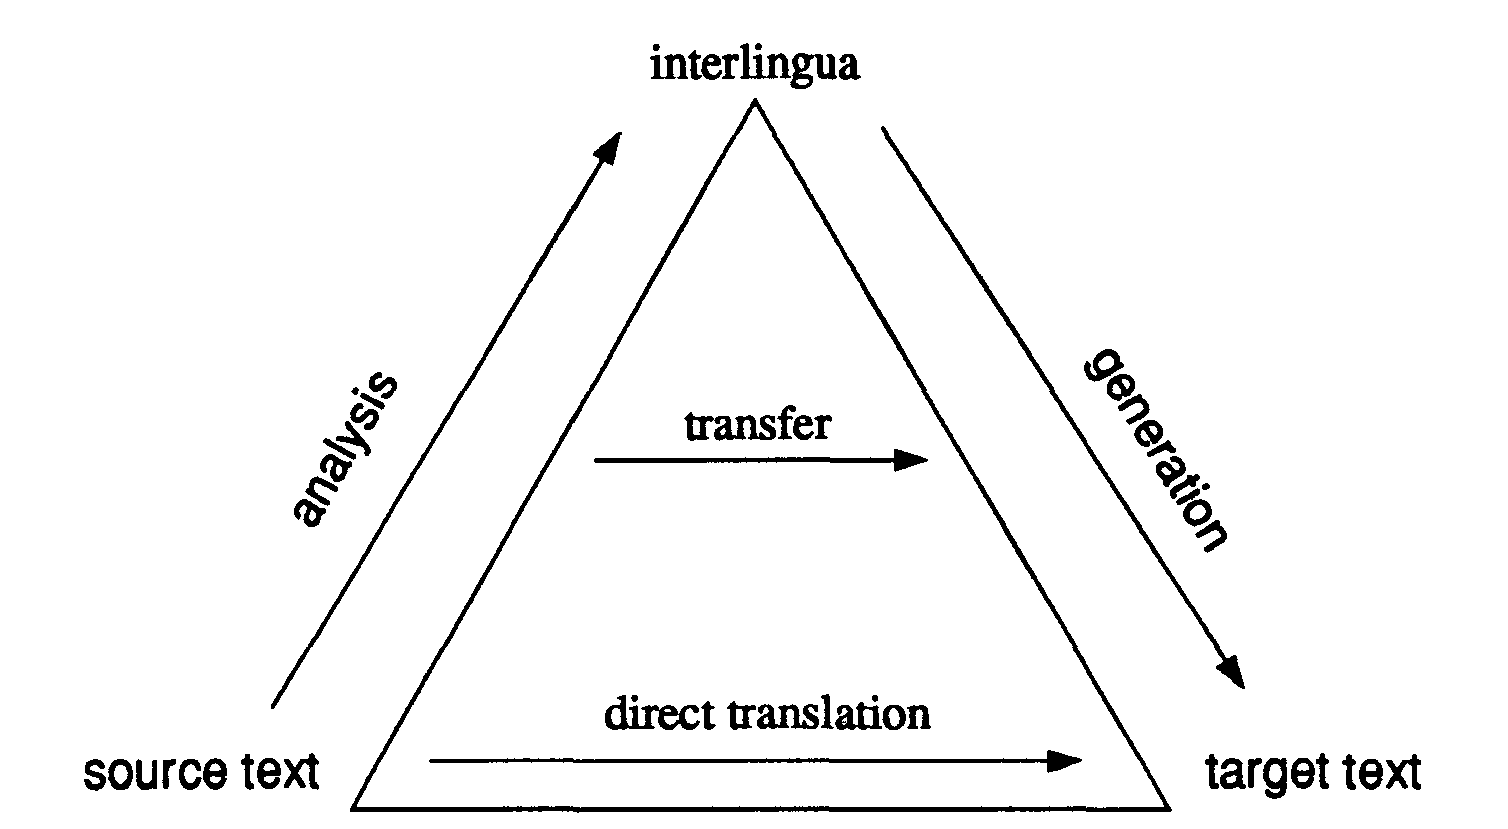
\includegraphics[scale=0.2]{translation_triangle.png}
\caption{Vauquois pyramid?}\label{fig:triangle}
\end{figure}

\section{Statistical MT}

In the 80's a new line of research was started, that was not primarily based on linguistic knowledge, but on large pairs of text that were translations of each other (parallel corpora). As many of the models developed then were based on analogy, finding examples in the corpus similar to fragments of the sentence to be translated and recombining them, this line of research is often called Example-Based Machine Translation (EBMT). Although in the beginning EBMT seemed to be a rival to the existing more linguistically oriented paradigm, soon people concluded that the two approaches were not actually conflicting and now most models combine the two approaches. The early EBMT models will not be further discussed here. Even though some of them have a nice theoretical founding (maybe mention the special case Furuse \& Iida's hierarchical phrases), most of them are computationally not executable and certainly not scalable. Exceptions to this are the corpus based models that do not match and recombine, but use the corpora to statistically decide on the parameters of their models. The results of early machine translation models, even though no linguistic knowledge was incorporated whatsoever, were a huge improvement over the rule-based models researchers had been developing before, and current state of the art machine translation models still make use of similar techniques. A brief introduction to early SMT models therefore belongs in a work like this.


%find in somers review if there were relevant models, transfer models, domain and results
% Really experimental: database size often not clear, sometimes just shown to work for one or two phenomena
% most methods not interesting for this work, some of them store treestructures and recombine
% Furuse & Iida’s (1992a, b) (isn't this just like hierarchical phrases
% Some approaches seem just not so worked out, and are later presented as 'new' (maybe also because of computational problems?
% Used when the rule based approach was to difficult.
% the “tree edit distance” (e.g. Noetzel & Selkow 1983; Zhang & Shasha 1997; see also Meyers et al. 1996, 1998) ??
% p 139: example based transfer

\subsection{Word-based models}

The idea to a statistical based was first introduced in 1988 by \citeauthor{brown1988statistical}.
Explain the idea behind word-based models.

\subsection{Phrase-based models}

%Zeg iets in de trant van: huge quality improvement
the IBM word based models still had the same drawbacks as the first generation of direct translation models: no structure or local context was considered and a large amount of natural language phenomena could therefore not be accounted for. The first phrase-based model (ref???) was a major leap forward. Keeping the generative model identical, using phrases instead of words as basic units of translation allowed the model to use local context during translation. Phrase based models can therefore capture (short) contiguous idiomatic translations, as well as small insertions and deletions and local reordering. (examples?) However, such models still suffer from the fact that no structure is assumed between the basic units of translation (not to mention the fact that phrase-based translation knows several practical problems). Some attempts to directly incorporate syntactical information in the models (for instance by restricting the phrases to be linguistic phrases) did not improve translation quality --> reinforcement of rule based models

% phenomena in scope of around 3 consecutive words (then data sparseness)


\subsection{Statistical Syntax-based Models}

%Maybe some more general introductiory sentences?
The new generation of 
%Synchornous context free grammars
% Can account for: non-contiguous phrases, global reordering, model structure

Over the last decade, an enormous amount of models have been presented, many of which were hybrid models combining several different strategies. In this section, the focus primarily lies on models that use transfer as strategy to generate translations. These models will be referred to as `syntax-based' models, as they consider the structure of the sentence. Note that in this term the meaning of the word `syntax' can be interpreted both formally and linguistically, and the syntactic analyses of sentences do thus not necessarily correspond to the analysis a linguist would give to the sentence. In this section, a number of syntax-based models will be discussed, decoding will receive no attention. Once again, no claim to completeness is made. 
%say something like: hard to compare results because of different elements?

%suffer from computational problems: minimal rules (more generalization, fewer rules, but not linguistically motivated), all rules (exponentially many --> size restriction)


\begin{enumerate}
\item hierarchical phrases (\cite{chiang2005hierarchical}), improvement over standard phrase based machine translation model, practical problems ($\mathcal{O}(n)$ possible rules) + probability model not clear
\item incorporation source language syntactical information
\item ITG Wu
\item what's in a translation rule \cite{galley2004s}
\end{enumerate}

\section{The theoretical backbone of transfer models}

As seen in the previous section, syntax-based models attempt to find structural representations of sentences in different languages and a function that maps the representations of sentences in one language to the representations of sentences in another if and only if the sentences are each others translation. That such representations and mappings do exist is implicitly assumed. The overarching assumption is equivalent to a the well known principle of compositionality of translation:

\begin{quote}
Two expressions are each others translation if they are built up from parts which are each other's translation, by means of translation-equivalent rules (ref??)
\end{quote}

Evidently, if translation between any two languages obeys this principle, representational systems and mappings between them can be found, but the implication in the other direction is also valid. CONVINCINGLY EXPLAIN WHY!
As mentioned before, the principle hinges on several smaller assumptions about both language and translation.

% Get link to next section

%What are the assumptions that are implicit in this principle?
% -translation is literal
% -language is compositional
% -languages have a similar semantical structure

%introduce grammar as term for obtaining representations, maybe I want to switch these two sections??

\subsection{Grammars}

One of the assumptions most obviously present in the principle of compositionality of translation is that languages itself are compositional. Compositionality is a property possessed by most designed languages. The meaning of an expression in a logical language, for instance can be unambiguously determined by considering the atoms and the rule used to combine them. For programming languages a similar statement can be made. As for translation, there exists a principle describing this property:

\begin{quote}
Meaning of an expression is a function of the meaning of its parts and syntactic rule by which they are combined \cite{partee1984compositionality}
\end{quote}

Although the compositionality of some parts of natural language is undeniable, we can understand sentences we have never heard because we know the words in it and we are familiar with the methods that can be used to combine them, many have argued against compositionality of natural language as a whole. Note that the principle as presented before is very unspecific, and its validity for a certain language is highly dependent on the notion of parts, meanings and rules in this language. A detailed description of the arguments in the compositionality debate will not add much to the current work, 
blabla explain why
%arguments often focus on rare exceptions and contextual ambiguities. function doesn't have to be bijective
%Explain that current work doesn't focus on resolving ambiguities, and also that such things are maybe different for translation?
% Take something from the \cite{janssen1996compositionality} article to explain that compositionality is quite strong, depending on the grammar and the building blocks --> idiomatic expressions
%An often heard counterargument is the existence of so called idiomatic expressions, whose meaning cannot be derived from the words in it.
%compositionality is formally quite strong

In this paper, \citeauthor{janssen1996compositionality} also shows that although not every grammar is suitable for compositional meaning assignment, the class of languages that can be analysed is not restricted, nor are the meanings that can be assigned: any recursively enumerable language can be generated by a compositional grammar, and any semantics can be dealt with in a compositional way. \textit{Finding} algebra's that describe the meaning and syntax of a language is of course not a trivial task.

\subsection{Mappings}

Apart from assumptions about the languages involved, the principle of compositionality of translation also makes assumptions about the translation process itself. First of all, it assumes that translation should not only preserve meaning, but also form (as much as possible). In other words, it assumes that translation is literal. Generally, this is helpful when deciding about the adequacy of a translation. An example that illustrates this is the following: \textit{all ravens are black} is an adequate translation of the Dutch \textit{alle raven zijn zwart}, but the logical equivalent sentence \textit{if something is not black it is not a raven} is not \citep{landsbergen1989power}.  However, even without regarding idiomatic translations, that will be considered later, a translator can have many reasons to prefer a more free translation, even if a literal alternative is present. Although this is a real issue in practice, machine translation is by far not developed enough to be concerned with style issues and throughout this paper will be assumed that translation is as literal as possible. A similar simplification is made regarding ambiguity ... (explain)
% say something about discussion compositionality of translation??
% then start the discussion with examples that show that translation is not 'compositional'

Example \cite{landsbergen1989power}: 


%%


% Wat moet er nog in het stuk hier:
% Iets over hoe idiomatische vertalingen hierin passen
% Aannames die gemaakt worden
% De kracht van compositioneel vertalen

%for more examples, refer to landsbergen

%Landsbergen also gives an example for which no compositional solution is found (cross the river swimming), explain that this is a theoretical problem rather than a practical one. Solution is not elegant, but a grammar automatically derived from a parallel corpus won't be elegant anyways :p



\chapter{An Empirical Study}

In articles about syntax-based translation models the assumptions discussed in the previous chapter are are rarely mentioned, let alone questioned. Moreover, the evaluation of the models presented is based on the performance of an implemented version of them that is often, due to computational reasons, not even completely equivalent to the version presented. Furthermore, the hybrid nature of models makes the evaluation of the transfer part even fuzzier, as it is not clear which parts of the model are responsible for the results. The current work deviates from this research, in presenting an exploration of the underlying assumptions. Such an analysis is of theoretical importance, but can also serve as an estimate of how far syntax-based translation models can actually bring us and possibly even give information on how to do so.

%anders
As mentioned before, there are several sub-assumptions to investigate. The primary focus of this paper is on algorithmically finding a source side representational system that could in theory be suitable for compositional translation, working from a translation corpus of parallel sentences. In contrast to earlier work on this topic, which will be discussed in section (ref section), we will not start out with a standard syntactic formalism and check its suitability as representational system. Rather, we will consider all possible structures of a sentence that satisfy the requirement that they allow compositional translation, and test if it is possible to extract a consistent set containing a unique structure for every sentence in the corpus.\footnote{Note that the only way to check if the corpus is indeed consistent is to find a labelling that can cover the whole corpus}. A detailed description of the analysis will presented in section (..), after a discussion of related literature.

\section{Related Work}

%Somehow introduce related work

%This section needs to be rewritten, but does say approximately what I want
\cite{fox2002phrasal} investigated if phrases that are constituents in the source sentence are coherent in the target sentence, by counting how often there was an overlap between the target side spans two phrases are translated in (the span of a phrase being defined as the pair [x,y] in which x is the minimum position a word in the span is aligned to, and y the maximum position. (anders) In other words, she tested the suitability of constituent grammars as a source side representation. 
% explain what exactly she did
% give a short summary of her results

A manual analysis of the head crossings in the S-alignment lead to the conclusion that most of the found crossings were caused by errors in parsing or translation (16 out of 86 and 5 out of 86, respectively), and non literal translations in cases a more literal version was also valid (29 our of 86).
% discuss what else she did
% short discussion of the results (and her manual analysis)
% ne ... pas causing errors even though this could be captured in a rule (or maybe say this only later?)

Another ... is the empirical study presented by \cite{hwa2002evaluating}. \citeauthor{hwa2002evaluating} empirically evaluate the \textit{Direct correspondence assumption (DCA)}, the assumption that for two sentences that are each others translation, the syntactic relations in one sentence directly map to the syntactic relations in the other.

 %Explain similarity with compositionality of translation principle
%Explain that Hwa argues that the DCA cannot account for some well known and fundamental linguistic facts
%Explain that this is also what they show
%Explain what she does after (making linguistic adaptations)
%Discuss results --> no bijective relation between dependeny parses


\section{This Work}

Also the current work will present an evaluation based on alignments. We will explain how by, starting with explaining the basic concepts used, and ending with a complete description of the process followed (anders).
consists of .. subsections blabla

\subsection{Alignments}

The precise definition of a word alignment used throughout this paper is the following:

\begin{definition}
Given a source sentence $s = s_0 \ldots s_n$ and its translation $t = t_0 \ldots t_m$, an alignment $a$ is a set of pairs $(x,y)$ with $x\in \{0,1,\ldots,n\}$ and $y\in \{0,1,\ldots,m\}$ such that $(x,y)\in a$ iff $s_x$ is translated into $s_y$.
\end{definition}

Words can align to several words on the other side, as well as none, which yields different types of alignments. A one to one alignment is an alignment in which no word or source or target side is aligned to more than one word, in a many-to-one alignment target words may have links to more than one source side position. The alignment in Figure \ref{fig:alignment} is a one-to-many alignment, as the word 'likes' is aligned to both 'houdt' and 'van', but no target position that has more than one link. (anders) The least restrictive kind of alignment is the many-to-many alignment, in which both source and target words may have multiple alignment links. An alignment in which the source and target words are in the same order is called a monotonic alignment. 

\begin{figure}[!ht]
\centering
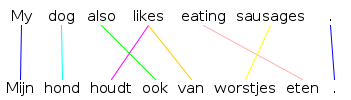
\includegraphics[scale=0.6]{alignment.png}
\caption{An alignment of the English sentence `My dog also likes eating sausages.' and its translation `Mijn hond houdt ook van worstjes eten'.%schrijf welke tool is gebruikt
}\label{fig:alignment}
\end{figure}

Naturally, a mapping from source to target words is not given for a translation\footnote{Even for humans it turns out to be a not so trivial task to find them (\cite{och2000improved})} and devising algorithms to find them is one of the problems in Machine Translation.
%Say that there are many approaches but that the IBM tools are still most commonly used
%Describe IBM alignments: they are a by-product of the word-based IBM models but only many-to-one alignments --> run in both positions and take union, intersection or use other heuristics to obtain alignment
%Tell that there are some manual corpora available (+references?)
%Maybe examples of problems in alignments


\subsection{Phrase Pairs}

The alignment of a parallel sentence restricts the space of parts possibly used in the translation. Analogous to the phrases used in the original phrase-based translation models \citep{och2004alignment}, a phrase pair is a pair of source and target spans [i,j] and [x,y], respectively, such that at least one word in [i,j] is aligned to at least one word in [x,y], and no words in [i,j] are aligned to words outside [x,y] and vise versa.(anders)The source sentence phrases consistent with the alignment are thus phrases whose translation is also a phrase. Note that in this context the word `phrase' denotes any arbitrary sequence of words that is contiguous, and is thus not restricted to linguistic phrases. For instance, the phrases consistent with the alignment in Figure \ref{fig:alignment} (the dot aside) are: ([0,0], [1,1], [2,3], [4,4], [5,5], [0,1], [2,3], [4,5], [1,3], [0,4], [2,5], [0,5]). In which [x,y] includes all words from position $x$ to position $y$. Note that the word 'like' does not form a phrase on its own, as it translates into two non-adjacent words in the Dutch target sentence. The number of phrases consistent with an alignment depends on the type of alignment and is largest in case of a monotone alignment, that does not restrict the set of possible phrases at all. A completely monotone alignment of a sentence of $n$ words has $\frac{n\times n+1}{2}$ phrases. Note that unaligned words can cause exponential growth in the number of phrases.
%I feel like something misses here
\cite{zhang2008extracting} presented an algorithm for efficiently extracting all tight phrases (i.e. phrases that do not start or end with an unaligned word) in $\mathcal{O}(n)$ time.

\subsection{Alignment Trees}

Now that the possible `parts' of the translation are defined, also the set of compositional structures according to which the sentence could have been translated. A completely specified translation structure is a tree covering the whole sentence, in which the nodes are phrases consistent with the alignment. We will call such trees alignment trees. Figure \ref{fig:alignment_tree} shows one of the possible alignment trees for the example alignment in figure \ref{fig:alignment}.

\begin{figure}
\Tree [.[0,6] [.[0,1] [.[0,0] my ] [.[1,1] dog ] ] [.[2,6] [.[2,4] [.[2,2] also ] [.[3,3] likes ] [.[4,4] eating ] ] [.[5,6] [.[5,5] eating ] [.[6,6] sausage ] ] ] ] ]
\caption{A possible alignment tree for the alignment of Figure \ref{fig:alignment} \label{fig:alignment_tree}}
\end{figure}

An alignment may have many different possible alignment trees. The number of alignment trees can be exponential (?) in the length of the sentence, if no restriction is placed on the branching factor of the nodes. Every alignment can be assigned at least one structure, that is completely flat.

%Maybe iets zeggen over hoeveel, en iets over empirische analyse Khalil en Gideon.

As mentioned in dunno chapter on statistical models factorizing alignments is blablabla

% mention some work on factorizing alignments (chiang, khalil, ...) 

\subsection{Hierarchical Alignment Trees}

In our evaluation we will consider all maximal trees recursively factorizing the alignment (anders), as presented by \cite{simaan2013hats2}.
Currently I really do not know what I need to write about HATs
At least write how HATs can account for phenomena as ne ... pas.


\subsection{Tree Selection}

We have now described the set of structures that we will investigate
Explain we want to pick one structure for each sentence, such that the set of structures for all sentences is consistent. 
Explain we will start out from the idea that we are supposed to have some idea about the semantical structure of sentences, say we will start out from dependency grammars. 
Explain that there may be several reasons that dependency structures depart from HATs, mention 


\chapter{Theory}

\section{Dependency Grammar}

%Introduction: maybe some history about dependency grammars and how they came about (refer to phrase structure grammars)

%Explain why dependency relations seems suitable for the task at hand: we want to see if predicate argument relations stay intact, dependencies are predicate argument relations
%Maybe also some arguments from other studies that support the suitability of dependency grammars (higher cohesion dependency grammars fox e.g, work quirk & menezes.

%Describe stanford dependency representation

The Stanford Dependency representation distinguishes five different styles. As an elaborate description of these styles, as well as an extensive list of the relations in all of them, can be found in the Stanford typed dependency manual \citep{de2008stanford}, in this thesis just a short summary will be given.
\paragraph{Basic Dependencies} The basic dependency style contains, as the name suggests, all the basic dependencies present in the sentence. A basic dependency structure is a fully connected projective dependency structure, that is, there are no crossing dependencies.
\paragraph{Collapsed dependencies} In the collapsed representation several dependencies involving function words are collapsed to get direct dependencies between content words. Furthermore, additional dependencies that break the tree structure are considered, which means the resulting dependency graph is not guaranteed to be acyclic or even a tree. There exist another 2 variants of the collapsed dependency representation, one in which conjunct dependencies are propagated, and one in which the dependencies that do not preserve the tree structure are omitted.
\paragraph{Non-collapsed dependencies} The last representation gives the basic dependencies as well as the extra ones which break the tree structure.

%Describe available parsers.
Zeg iets over de beschikbare parsers \cite{de2006generating}
%Probeer misschien nog wat andere literatuur te vinden over dependency grammar

\section{The Best Tree}

Describe that we need a way to decide how good a tree is and that there are different ways to do that. Present evaluation metrics.

\subsection{Shared Notation}

Firstly, we will present some notation that is shared along the different metrics.

\begin{notion}
$T_d$ will refer to a dependency tree of a sentence $s = w_1 \dots w_n$, formed by a set of dependencies $D = \{ (i,j) |$ there is a dependency arrow from word $w_i$ to word $w_j \}$.
\end{notion}

\begin{notion}
If $T_d$ is a dependency tree for $s$, $w$ is a word in $s$ and $i$ and $j$ are the maximum and minimum positions, respectively, that can be reached from $w$ by following the directed dependency arrows. Then span($w$) = $[i,j]$.
\end{notion}

\begin{notion}
$T_a$ will be used to refer to an alignment tree of a sentence $s = w_1 \dots w_n$. The label $i-j$ will refer to the node that dominates span $[i,j]$. The highest node of $T_a$ will be denoted with $N_{T_a}$
\end{notion}

\begin{notion}
Let $T_d$ be a dependency tree with dependencies $D$, Then $D' = \{ (i,\textrm{span}(j))$ $|$ $D(i,j) \land 1 \leq i,j \leq n \}$ is the set in which each dependent is replaced by its span.
\end{notion}

\begin{notion}
If $N$ is a node in a tree $T_a$, $C_N$ denotes the set of child constituents of this node. If node $N$ dominates words $i$ to $j$ in $s$, then $dom(N)= [i,j]$
\end{notion}

\subsection{Metric 1}

A dependency tree $T_d$ tells us exactly of which are the smaller parts of the sentence and how they are combined to obtain the complete sentence. Consider for instance the dependency tree of the sentence "My dog also likes eating sausage" (Figure \ref{fig:deptree1}).

\begin{figure}[!h]\label{fig:deptree1}
\centering
\begin{dependency}[theme=simple]%[hide label]
\begin{deptext}[column sep=.5cm, row sep=.1ex]
%PRP\$ \& NN \& RB \&[.5cm] VBZ \& VBG \& NN \\
My \& dog \& also \& likes \& eating \& sausage \\
\end{deptext}
\deproot{4}{}
\depedge{2}{1}{poss}
\depedge{4}{2}{nsubj}
\depedge{4}{3}{xvmod}
\depedge{4}{5}{xcomp}
\depedge{5}{6}{dobj}
\end{dependency}
\caption{Stanford Dependency Tree}
\end{figure}

\noindent The dependency tree tells us that 'likes' is the head word of the sentence, and that the sentences is composed of 4 parts: the head 'likes', its modifier 'also', its noun subject whose head is 'dog' and the open clausal complement whose head is 'eating'. The complement and subject are further divisible in, 'My' and 'dog', and 'eating' and 'sausage', respectively. Intuitively, for every relation in the dependency parse, we can check whether this relation exists in an alignment tree $T_a$, by checking if the word and its depending subtrees are siblings in $T_a$. The evaluation metric used in this first experiment is based upon this intuition.

\begin{metric}\label{m1}
Let $s = w_1 w_2 \dots w_n$ be a sentence, and $T_d$ and $T_a$ its dependency tree and an alignment tree, respectively. The score of $T_a$ is defined as the score of its highest node $N_{a}$:

$$
E(N_a,D) = \sum_{c\in C_{N_a}} E(c,D)+ \sum_{c_1\in C_{N_a}} \sum_{c_2\in C_{N_a}} B(c_1,c_2)
$$

\noindent With base case $E(N,D) = 0$ and $B(c_1,c_2) = 1$ iff  $(c_1,c_2)\in D'$. Dividing the resulting score by $|D'|$ will result in a normalized score.
\end{metric}

\noindent  Note if this definition is strictly followed more than half of the sibling checks is redundant, an algorithm computing the score of a tree would not have to perform them all.

\subsection{Metric 2}

Explain that metric 1 reflects the similarity with the dependency parse, rather than giving a reasonable measure of compositionality. Explain why this is, that a part of the score can trivially be reached by just making a flat tree. Explain how to fix this. Explain that evaluation metric 2 won't alter the ordering of the trees, just their scores.
Explain that metric 2 thus just differs in the set of relations it considers: instead of considering all relations from the dependency parse, it only considers the relations that reflect compositionality, which captures the intuition that completely flat trees should be assigned a 0 score. Note that this means that this therefore does not alter the ranking of the trees set by metric 1, it just alters the scores associated with the trees.

\begin{metric}\label{m2}
Let $s = w_1 w_2 \dots w_n$ be a sentence, and $T_d$ and $T_a$ its dependency tree and an alignment tree, respectively. The score of $T_a$ is defined as the score of its highest node $N_{a}$:

$$
E(N_a,D) = \sum_{c\in C_{N_a}} E(c,D)+ \sum_{c_1\in C_{N_a}} \sum_{c_2\in C_{N_a}} B(c_1,c_2)
$$

\noindent With base case $E(N,D) = 0$ and $B(c_1,c_2) = 1$ iff  $|dom(c_2)| > 1 \land (c_1,c_2)\in D'$ the part of the sentence covered by $c_2$. Dividing the resulting score by $|D'|$ will result in a normalized score.
\end{metric}

Note that normalizing the score will sometimes result in zero division for shorter sentences whose dependency parses display no compositional structure, in this cases we will define the score of the sentence to be 0.

%CHAPTER DESCRIBING THE IMPLEMENTATION OF THE EXPERIMENTS

\chapter{Implementation}
\label{chapter:impl}
%Alternative title: compositionality in practice
Describe that recursive alignment trees are very useful for investigating the recursive properties of translation. Describe empirical research \cite{simaan2013hats}.\\
Describe that in this work we will use the structures for investigating the preservation of predicate argument structures, as extracted from dependency parses. Explain that we let go of the restriction that the HATs should be minimally branching (+reason), say something about that we only look at the tree structure and not at the reordering, as this is for the theoretical question unimportant.
Unaligned words also all considered. Say that this significantly increases the complexity of the task, but that this is less of a problem as the purpose is analysis, thus we only have to do it once.



\section{Setup}

Explain that the main framework scores an alignment according to a given set of preferred relations between nodes that are siblings in the tree, or nodes that are mother and child. Explain that it is designed to be easily extendible for testing different properties of the tree.

Explain that tests were conducted with different evaluation metrics, information about which can be found in the description of the experiments.

%Do not know what level of detail is required here...
Briefly discuss how: for each alignment a grammar is created that uniquely generates all Recursive Alignment Trees. The different productions of this grammar are assigned a score proportional to the preferred number of mother child relations that it generates. (similar to a probability, but not the same). A parser is used to find the optimal alignment tree (i.e. the alignment tree with the highest number of preferred mother child relations), and its score.
%Maybe say something about the scoring and how different things can be tested but that one needs to think about scores for the productions


\section{Implementation}

Open source implementation that consists of different parts

\begin{itemize}
\item the part that deals with the dependency relations, extracts different relations from them and assigns labels to spans
\item part that generates the context free grammars, details about this is implemented? graph approach, spans found by an algorithm similar to Zhangs.. def of phrases is slightly different, an emtpy node can also be a phrase.
\item parser, external viterbi parser from nltk toolkit \citep{bird2009natural}, slightly adapted such that it can dael with scores that are not probabilities 
\end{itemize}

The only thing that is thus required is an evaluation metric

%Show that graph algorithm is sound and complete

\chapter{Results}

% What I want to describe now: ran test experiments on a small dataset, results: HATs do not capture compositionality as in the dependency parses, a small problem are the alignments, but a bigger problem is that the structure from the compositionality derived from the dependency parses is not minimally branching (test with ALL trees)
% but our goal is to find a consistent set of structures (i.e. consistently label them), so maybe we can do it diffently
% Investigate which relations ARE preserved, investigation on bigger dataset, find which relations are preserved and which aren't and see which ones are preserved an which ones aren't, maybe we can now investigate new labels?

We conducted experiments on both manual and automatically aligned corpora. The dataset used in the experimens can be found in table \ref{table:datasets}

\begin{table}\label{table:datasets}
\begin{tabular}{cccc}
Name corpus & section & size & alignments\\
\end{tabular}
\caption{Datasets}
\end{table}

\section{Datasets}

Describe which experiments were done with which dataset. Describe
Tell something about datasets, preparation, blabla
%Denk dat ik dit toch net iets anders wil doen, zodat ik alle resultaten in 1 tabel kan zetten enzo

\section{Experiments}

Describe which experiments were done (with which datasets, which metrics..)

\section{Results}

\begin{table}\label{table:scores}
\begin{tabular}{llll}
Experiment 1 & metric 1 & dataset 1 & 0.84\\
Experiment 2 & metric 2 & dataset 1 & 0.52\\
Experiment 3 & metric 2 & dataset 2 & 0.79\\
\end{tabular}
\caption{Average sentence score of corpus (vul in) according to different metrics.}
\end{table}


The average sentence score of this corpus is 0.830827979565.

\section{Discussion}

Discussion of the results of the experiments, analysis of the results

At the first sight, the results of experiment 1 seem very promising: on average over 80\% of the dependency relations are supported by the alignment. However, the trees in the outputted corpus seems strikingly flat, even for long sentences. Although one could argue that this is also compositional in some aspect, it is definitely not the kind of compositionality that is interesting in the light of Machine Translation. The obtained score might have reflected the similarity with the dependency parses well, but seems no good measure for compositionality. This is mainly caused by the fact that not all relations in the dependency parse actually reflect compositionality. The average fraction of relations that express word to word relations over the entire corpus is 0.56 %(this is not just over the 46 sentences parsed, fix that!)
, which means that a score of 0.56 could be obtained by simply assigning every sentence in the corpus a completely flat tree. Experiment 2 addresses this problem, altering the evaluation metric such that the score of an alignment tree primarily reflects compsitionality, rather than similarity with the dependency tree of the sentence.


\subsection{Analysis}

There are 4 main reasons that could result in a low score for evaluation metric 2:
\begin{enumerate}
\item Errors in the translation or non literal translation;
\item Errors in the alignment;
\item Error in the dependency parse;
\item The sentence cannot be compositionally translated.
\end{enumerate}

For X scored sentences a tree with a score higher than 0.70 was found. Manual analysis of the other 46-X analysed sentences (\ref{tab:class} showed that most of the low compositionality scores weren't for lack of possible compositional translations, but were merely due to translation errors, errors in sentence alignment and for the larger part errors in the alignment.

\begin{table}[!h]\label{tab:class}
\begin{tabular}{|l|l|}
\hline
Translation Error & \\
Alignment Error & \\
Parse Error &\\
No Compositional translation possible & \\
\hline
\end{tabular}
\caption{Manual analysis of the X scored}
\end{table}

If the lack of compositionality found in the corpus was really caused by poor automatic alignments, one would expect the score of a corpus scored manually to be higher. This hypothesis is tested in experiment 3.

Een stuk hoger indeed, analysis of de bomen lager dan 0.7 in deze dataset

Wat zijn mogelijke opties voor extensie?

\chapter{Discussion and Future Work}

short summary of findings and what they mean

future work: source reordering, treebank to learn translation structure


\chapter{Conclusion}

%THINGS I SHOULDN'T FORGET TO MENTION!

% zeg iets over dat we op deze manier nicely omgaan met phrasal translations

% put statistics about the data, the dependency parses, everything

% ook wat analyses over complexiteit e.d. max grootte van de grammatica's dat soort zaken

% niet zo tevreden over hoe dependency grammars met conjunction omgaan, collapsed dependencies doen dit wel beter trouwens, misschien moet ik daar nog eens naar kijken. Collapsed dependencies doen soms ook al wat werk met idiom (zie tabel 3)

%Maybe moet ik nog iets zeggen over dat compositionaliteit aangenomen wordt in veel systemen (e.g. rule-based systemen)

%Geen enkel vertaalsysteem vertaalt een zin 'in zijn geheel', altijd in stukken

% Bouw iets in in dat dependency programma dat oneindige recursie tegengaat

% Bouw meer checks in die kijken of de input wel consistent is

% Zeg ergens iets over dat vertalers ook vaak de keuze maken om iets niet letterlijk te vertalen, maar dat we er hier vanuit gaan dat dit wel gebeurt (of iig zo letterlijk mogelijk)

%Say something about partitioning problem with phrase based MT??

% Make a comment about reordering?

% A compositional approach ideally takes care of several problems at the same time

% Ergens moet ik ook nog de vraag stellen of we de semantiek en de syntax echt apart nodig hebben (zoals in Rosetta). 

\bibliography{thesisDH}

\end{document}
